\documentclass[12pt,letterpaper]{article}
\usepackage{amsmath,amsthm,amsfonts,amssymb,amscd}
\usepackage{fullpage}
\usepackage{graphicx}
\usepackage{lastpage}
\usepackage{enumerate}
\usepackage{fancyhdr}
\usepackage{hyperref}
\usepackage{mathrsfs}
\usepackage{xcolor}
\usepackage[margin=3cm]{geometry}
\setlength{\parindent}{0.0in}
\setlength{\parskip}{0.05in}

% Edit these as appropriate
\newcommand\course{STA571/CS590.01}
\newcommand\semester{Spring 2014}                   % <-- current semester
\newcommand\papertitle{Bayesian Hierarchical Clustering}                          % <-- paper title
\newcommand\authoryear{Heller and Ghahramani, ICML, 2005}
\newcommand\yourname{Matt Dickenson}                % <-- your name
\newcommand\login{mcd31}                            % <-- your NetID
\newcommand\hwdate{Due: 24 February, 2014}           % <-- HW due date


\pagestyle{fancyplain}
\headheight 60pt
\chead{The Indian Buffet Process\\ ~\\}
\lhead{\small \yourname\ \texttt{\login}\\\course}
\rhead{\small \hwdate}
\headsep 10pt

\begin{document}

% \noindent \emph{Homework Notes:} 

The following code was used to implement a generative model for the Indian Buffet Process. Example matrices generated from this code are displayed below. 

\lstinputlisting[caption=IBP code, language=R, lastline=56]{2-24-homework.R}

How do the results vary with $\alpha$ and $n$? As $\alpha$ increases, so does the average number of dishes per customer and the total number of non-zero columns $K_+$ (compare Figures \ref{alpha5n5} and \ref{alpha5n10} to Figures \ref{alpha10n5} and \ref{alpha10n10}). Because of the way that the Poisson parameter is reduced with each new customer, $K_+ \sim \text{Poisson}(\alpha H_N)$ (where $H_N$ is the $N^{th}$ harmonic number). By exchangeability, the number of dishes on each customer's plate is distributed Poisson($\alpha$).

When $n$ increases but $\alpha$ is held constant, the resulting matrix is more sparse (compare Figures \ref{alpha5n5} and \ref{alpha10n5} to Figures \ref{alpha5n10} and \ref{alpha10n10}). The matrix $\bf{Z}$ remains sparse because the effective dimensions of $\bf{Z}$ are $N \times K_+$, and the expected number of entries is $N\alpha$.

\begin{figure}[h!]
\begin{center}
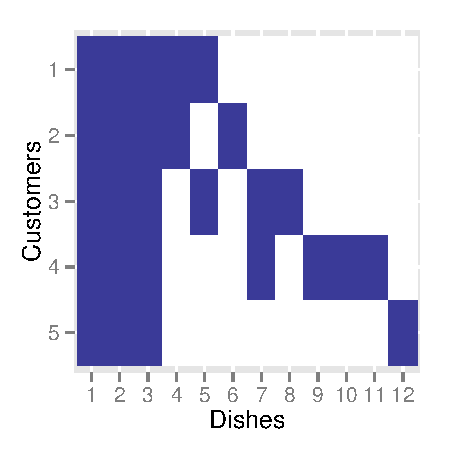
\includegraphics{alpha5n5.pdf}
\caption{Example Matrix Generated from IBP with $\alpha=5, n=5$}
\label{alpha5n5}
\end{center}
\end{figure}

\begin{figure}[h!]
\begin{center}
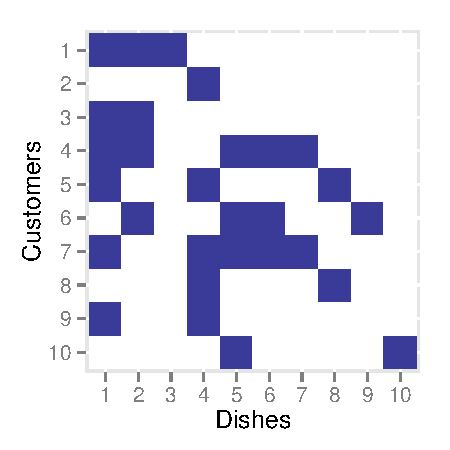
\includegraphics{alpha5n10.pdf}
\caption{Example Matrix Generated from IBP with $\alpha=5, n=10$}
\label{alpha5n10}
\end{center}
\end{figure}

\begin{figure}[h!]
\begin{center}
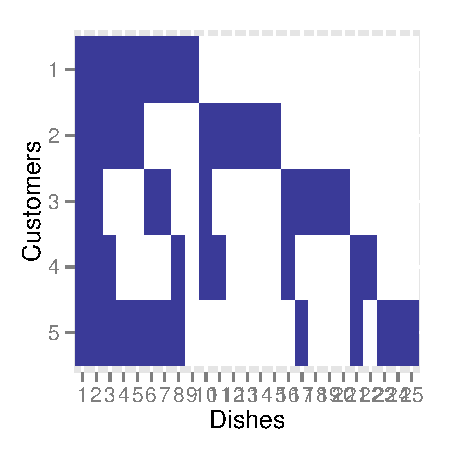
\includegraphics{alpha10n5.pdf}
\caption{Example Matrix Generated from IBP with $\alpha=10, n=5$}
\label{alpha10n5}
\end{center}
\end{figure}

\begin{figure}[h!]
\begin{center}
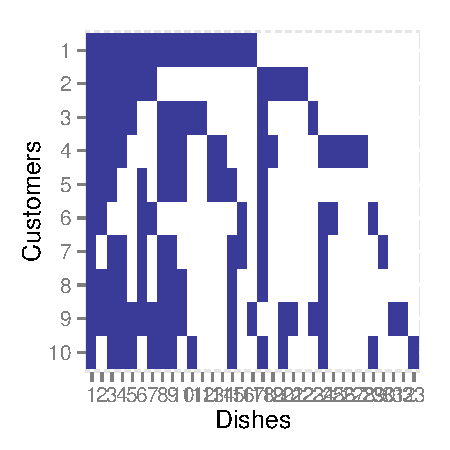
\includegraphics{alpha10n10.pdf}
\caption{Example Matrix Generated from IBP with $\alpha=10, n=10$}
\label{alpha10n10}
\end{center}
\end{figure}


\end{document}
